\pdfoutput=1
\documentclass[10pt,twocolumn,letterpaper]{article}
\usepackage[T1]{fontenc}
\usepackage[utf8]{inputenc}
\usepackage{mathptmx}
\usepackage{microtype}
\usepackage[margin=0.75in,columnsep=0.28in]{geometry}
\usepackage{amsmath,amssymb}
\usepackage{graphicx}
\usepackage{booktabs}
\usepackage{array}
\usepackage{xcolor}
\usepackage{tikz}
\usetikzlibrary{positioning,arrows.meta,fit}
\usepackage[numbers,sort&compress]{natbib}
\usepackage[colorlinks=true,linkcolor=blue!60!black,citecolor=red!60!black,urlcolor=blue!60!black]{hyperref}
\usepackage{titlesec}
\usepackage{abstract}
\usepackage{caption}
\usepackage{fancyhdr}
\captionsetup{font=small,labelfont=sc,labelsep=colon,justification=justified}

% Section style modeled on the APS layout of the reference preprint
\renewcommand{\thesection}{\Roman{section}}
\renewcommand{\thesubsection}{\Alph{subsection}}
\titleformat{\section}{\centering\normalsize\bfseries\MakeUppercase}{\thesection.}{0.6em}{}
\titleformat{\subsection}{\centering\normalsize\bfseries}{\thesubsection.}{0.5em}{}
\titlespacing*{\section}{0pt}{1.4ex plus .3ex}{0.8ex}
\titlespacing*{\subsection}{0pt}{1.1ex plus .2ex}{0.6ex}
\renewcommand{\figurename}{FIG.}
\renewcommand{\tablename}{TABLE}
\renewcommand{\thetable}{\Roman{table}}
\setlength{\parskip}{0pt}
\raggedbottom
\makeatletter\renewcommand\p@subsection{\thesection\,}\makeatother

% Generated by analysis/make_numbers.py. Do not edit by hand.
\newcommand{\ModelForm}{3PH}
\newcommand{\CvRmse}{7.9}
\newcommand{\RSq}{0.988}
\newcommand{\SlopeT}{42.3}
\newcommand{\AdjBaseline}{45,617}
\newcommand{\ReportingUse}{38,737}
\newcommand{\AvoidedTherms}{6,879}
\newcommand{\FracSav}{15.1}
\newcommand{\FSU}{34.2}
\newcommand{\AbsUnc}{2,352}
\newcommand{\TrueAvoided}{6,629}
\newcommand{\TrueAdjBaseline}{44,191}
\newcommand{\ErrTherms}{251}
\newcommand{\ErrPct}{3.8}
\newcommand{\AdjBaseErrPct}{3.2}
\newcommand{\EquationIntercept}{43.00}
\newcommand{\EquationSlope}{6.37}
\newcommand{\EquationCp}{57}
\newcommand{\OnePct}{98.3}
\newcommand{\TwoPct}{113.6}
\newcommand{\PlannedUnit}{26.43}
\newcommand{\ActualUnit}{28.56}
\newcommand{\UnitRatio}{8.1}
\newcommand{\CvMean}{69.5}
\newcommand{\RsqMean}{$-$0.025}
\newcommand{\TMean}{n/a}
\newcommand{\BicMean}{380.9}
\newcommand{\CvTwoP}{17.3}
\newcommand{\RsqTwoP}{0.939}
\newcommand{\TTwoP}{18.8}
\newcommand{\BicTwoP}{316.3}
\newcommand{\CvThreePH}{7.9}
\newcommand{\RsqThreePH}{0.988}
\newcommand{\TThreePH}{42.3}
\newcommand{\BicThreePH}{280.8}
\newcommand{\CvFourP}{8.0}
\newcommand{\RsqFourP}{0.988}
\newcommand{\TFourP}{0.7}
\newcommand{\BicFourP}{283.4}
\newcommand{\CvFiveP}{8.4}
\newcommand{\RsqFiveP}{0.988}
\newcommand{\TFiveP}{0.1}
\newcommand{\BicFiveP}{287.5}
\newcommand{\OptASavings}{28,392}
\newcommand{\OptAUnc}{717}
\newcommand{\OptARel}{2.5}
\newcommand{\OptABase}{49,348}
\newcommand{\OptARep}{20,956}
\newcommand{\LccBase}{1,287,460}
\newcommand{\LccAlt}{1,135,786}
\newcommand{\NetSavings}{151,675}
\newcommand{\AddedInv}{119,656}
\newcommand{\OpSav}{271,331}
\newcommand{\SIR}{2.27}
\newcommand{\AIRR}{6.4}
\newcommand{\SPB}{7.8}
\newcommand{\DPB}{9.0}
\newcommand{\LccBInitial}{0}
\newcommand{\LccBReplacement}{74,994}
\newcommand{\LccBResidual}{0}
\newcommand{\LccBEnergy}{1,099,281}
\newcommand{\LccBOmr}{113,185}
\newcommand{\LccBTotal}{1,287,460}
\newcommand{\LccAInitial}{196,500}
\newcommand{\LccAReplacement}{7,702}
\newcommand{\LccAResidual}{9,552}
\newcommand{\LccAEnergy}{871,483}
\newcommand{\LccAOmr}{69,653}
\newcommand{\LccATotal}{1,135,786}
\newcommand{\DueDate}{2026-03-31}
\newcommand{\NsLow}{100,413}
\newcommand{\NsHigh}{202,937}
\newcommand{\SirLow}{1.84}
\newcommand{\SirHigh}{2.70}
\newcommand{\BeRate}{9.2}
\newcommand{\NsZeroGas}{7,924}
\newcommand{\NsPerTherm}{20.90}
\newcommand{\BeYears}{10}
\newcommand{\GasSavPV}{143,751}
\newcommand{\McReps}{2,000}
\newcommand{\ScanReps}{500}
\newcommand{\McMeanErr}{$-$17}
\newcommand{\McRmse}{1,613}
\newcommand{\McSdErr}{1,613}
\newcommand{\McMeanTrue}{6,596}
\newcommand{\McMeanUnc}{2,770}
\newcommand{\McMedFsu}{41.7}
\newcommand{\McPass}{72.7}
\newcommand{\McFsuOk}{72.7}
\newcommand{\McMaxNmbe}{1.5\times 10^{-13}}
\newcommand{\McCovEighty}{79.8}
\newcommand{\McCovNinety}{90.0}
\newcommand{\McCovNinetyFive}{94.6}
\newcommand{\McFormThreePH}{87.6}
\newcommand{\McFormFourP}{11.6}
\newcommand{\McFormFiveP}{0.8}
\newcommand{\McFormTwoP}{0.0}
\newcommand{\OaReps}{20,000}
\newcommand{\OaSd}{0.20}
\newcommand{\OaCovEighty}{80.1}
\newcommand{\OaCovNinety}{90.1}
\newcommand{\OaCovNinetyFive}{95.0}
\newcommand{\OaMedRel}{2.7}
\newcommand{\NonposFive}{10.6}
\newcommand{\NonposTen}{0.8}
\newcommand{\NonposNoise}{7.8}
\newcommand{\BeforeThreePH}{76.5}
\newcommand{\BeforeNonThree}{23.5}
\newcommand{\AfterNonThree}{12.4}
\newcommand{\BeforeCovNinety}{89.5}
\newcommand{\BeforeRmse}{1,649}
\newcommand{\BeforeCovFive}{86.0}
\newcommand{\BeforeUndefFive}{11.0}
\newcommand{\BeforeCovNoise}{87.4}
\newcommand{\CovNoiseThirtySix}{91.6}
\newcommand{\UfFivePBefore}{56.0}
\newcommand{\UfFivePAfter}{30.7}
\newcommand{\UfFivePRmseChange}{1.8}
\newcommand{\UfFourPRmseChange}{$-$0.7}
\newcommand{\UfFivePCovAfter}{92.7}
\newcommand{\UfFivePCovBefore}{93.3}
\newcommand{\McSeRef}{0.7}
\newcommand{\McSeScan}{1.3}
\newcommand{\McMedCv}{9.6}
\newcommand{\CovFrFive}{91.6}
\newcommand{\CovFrTwenty}{91.6}
\newcommand{\CovYrOne}{86.6}
\newcommand{\CovYrThree}{93.2}
\newcommand{\CovYrOneEighty}{74.6}
\newcommand{\PassFrTen}{27.2}
\newcommand{\PassFrTwenty}{94.2}
\newcommand{\PassNoiseTwentyFour}{9.4}
\newcommand{\CvOkNoiseThirtySix}{19.6}
\newcommand{\MedFsuFive}{106.3}
\newcommand{\MedFsuThirty}{20.9}
\newcommand{\RmseYrOne}{2,365}
\newcommand{\RmseYrThree}{1,499}
\newcommand{\RmseNoiseSix}{781}
\newcommand{\RmseNoiseThirtySix}{4,709}
\newcommand{\CovFormThreePH}{90.8}
\newcommand{\RmseFormThreePH}{1,602}
\newcommand{\MeanErrFormThreePH}{$-$31}
\newcommand{\NFormThreePH}{1,752}
\newcommand{\CovFormFourP}{84.9}
\newcommand{\RmseFormFourP}{1,698}
\newcommand{\MeanErrFormFourP}{70}
\newcommand{\NFormFourP}{232}
\newcommand{\CovFormFiveP}{87.5}
\newcommand{\RmseFormFiveP}{1,534}
\newcommand{\MeanErrFormFiveP}{275}
\newcommand{\NFormFiveP}{16}
\newcommand{\BeforeAfterRows}{%
Selects 3PH (\%) & 76.5 & 87.6 \\
Selects 4P (\%) & 19.7 & 11.6 \\
Selects 5P (\%) & 3.8 & 0.8 \\
Coverage at 90\% (\%) & 89.5 & 90.0 \\
RMSE (therms) & 1,649 & 1,613 \\
\multicolumn{3}{@{}l}{\emph{Weak or noisy savings, coverage at 90\% (\%)}} \\
$F_{\rm true}=5\%$ & 86.0 & 91.6 \\
$\sigma=36$ & 87.4 & 91.6 \\
No uncertainty reported, $F_{\rm true}=5\%$ (\%) & 11.0 & 0.0 \\
\multicolumn{3}{@{}l}{\emph{True model 4P, 300 replications}} \\
Selects 4P (\%) & 70.0 & 72.0 \\
Coverage at 90\% (\%) & 92.3 & 92.7 \\
RMSE (therms) & 1,512 & 1,501 \\
\multicolumn{3}{@{}l}{\emph{True model 5P, 300 replications}} \\
Selects 5P (\%) & 56.0 & 30.7 \\
Coverage at 90\% (\%) & 93.3 & 92.7 \\
RMSE (therms) & 1,529 & 1,556 \\}
\newcommand{\ScanRows}{%
Reference & $-$17 & 1,613 & 41.7 & 79.8 & 90.0 & 94.6 & 72.7 & 0.0 \\
\multicolumn{9}{l}{\emph{Savings fraction $F_{\rm true}$}} \\
5\% & $-$18 & 1,686 & 106.3 & 80.2 & 91.6 & 95.6 & 1.4 & 10.6 \\
10\% & $-$18 & 1,686 & 61.4 & 80.2 & 91.6 & 95.6 & 27.2 & 0.8 \\
20\% & $-$18 & 1,686 & 31.4 & 80.2 & 91.6 & 95.6 & 94.2 & 0.0 \\
30\% & $-$18 & 1,686 & 20.9 & 80.2 & 91.6 & 95.6 & 100.0 & 0.0 \\
\multicolumn{9}{l}{\emph{Noise s.d. $\sigma$ (therms/day)}} \\
6 & 12 & 781 & 21.7 & 83.8 & 91.0 & 95.2 & 100.0 & 0.0 \\
24 & 37 & 3,126 & 84.3 & 82.8 & 91.6 & 95.4 & 9.4 & 1.6 \\
36 & 59 & 4,709 & 120.3 & 81.6 & 91.6 & 95.0 & 2.8 & 7.8 \\
\multicolumn{9}{l}{\emph{Baseline length (months)}} \\
12 & 80 & 2,365 & 45.3 & 74.6 & 86.6 & 93.8 & 60.6 & 0.0 \\
36 & 59 & 1,499 & 41.7 & 84.8 & 93.2 & 97.0 & 76.8 & 0.0 \\}
\newcommand{\FormRows}{%
Reference & 0.0 & 87.6 & 11.6 & 0.8 \\
$\sigma=6$ & 0.0 & 87.8 & 11.2 & 1.0 \\
$\sigma=36$ & 19.4 & 66.6 & 14.0 & 0.0 \\
12-month baseline & 0.0 & 79.6 & 18.8 & 1.6 \\
36-month baseline & 0.0 & 92.0 & 7.8 & 0.2 \\}

\newcommand{\draftmark}{}
\newcommand{\code}[1]{\texttt{#1}}

\pagestyle{fancy}
\fancyhf{}
\fancyhead[R]{\small\thepage}
\fancyhead[L]{\small\draftmark}
\renewcommand{\headrulewidth}{0pt}

\begin{document}

\twocolumn[
\begin{@twocolumnfalse}
\begin{center}
{\large\bfseries MUNI-LCC: An Open Toolkit Linking Measured Energy Savings, Life-Cycle Cost, and Federal Performance Reporting for Municipal Energy Projects\par}
\vspace{0.9em}
Stephen Olumide Akindipe\,\href{https://orcid.org/0000-0002-1846-9662}{
\includegraphics[height=0.8em]{figs/orcid.pdf}}\,$^{1}$\par
\vspace{0.3em}
{\small\itshape $^{1}$Independent Researcher, Albany, NY, USA\par}
{\small Correspondence: \href{mailto:oluakins1108@gmail.com}{oluakins1108@gmail.com}\par}
\vspace{0.4em}
\vspace{0.8em}
\begin{minipage}{0.86\textwidth}
\small

Energy upgrades and retrofits in small and mid-sized municipalities are funded through federal and state awards. Recipients of federal awards must report project accomplishments against award objectives, provide reasons for objectives not met, and account for any cost overruns or high unit costs pursuant to 2 CFR 200.329. The existing methods for evaluating savings over the project's lifespan are standardized and mostly prepared through the support of a consultant or a licensed software. This financial implication creates a burden for municipalities with budget constraints. MUNI-LCC addresses this challenge: It is an open-source python toolkit that implements Options A and C of the International Performance Measurement and Verification Protocol as defined in the U.S. Department of Energy FEMP M\&V Guidelines Version 5.0. It implements life-cycle cost analysis consistent with ASTM E917 through the NIST Handbook 135 framework and integrate the content elements of 2 CFR 200.329 to ensure accurate reporting. MUNI-LCC introduces a distinguishing feature whereby verified quantities directly feed the life-cycle cost study to ensure the net savings, savings-to-investment ratio, and unit cost reported to the sponsor is computed from the metered savings. 

Validated using a synthetic worked example with a known answer, a \ModelForm{} change-point baseline (CV(RMSE) \CvRmse\%, $R^2=\RSq$) yields \AvoidedTherms{} therms of avoided gas use against a true \TrueAvoided{} therms, inside the 90\% uncertainty of $\pm$\AbsUnc{} therms. In \McReps{} Monte Carlo replications of the same data-generating process, the ASHRAE Guideline 14 uncertainty approximation applied for Option C attains empirical coverage of \McCovNinety\% at a nominal 90\%, and mean estimation error is \McMeanErr{} therms. Outcome of these tests spurred two changes in version 0.1.1: information-criterion model selection and an uncertainty reported for any sign of savings, without altering the published result of the worked example. Sensitivity scans demonstrates how measured-savings uncertainty and the discount rate propagate to net savings. The toolkit is released under the MIT license and archived on Zenodo.\par\vspace{0.4em}
\textbf{Keywords:} measurement and verification, IPMVP, life-cycle cost analysis, change-point regression, savings uncertainty, municipal energy, Uniform Guidance, open-source software
\end{minipage}
\end{center}
\vspace{1.2em}
\end{@twocolumnfalse}
]

\section{Introduction}

Energy efficiency and heating-system upgrades conducted on public or municipal buildings are often funded through various financial mechanisms, including local capital budgets, utility programs, and grants from federal and state agencies. For projects funded through federal awards, recipients are required to provide a program performance report to maintain compliance with the Uniform Guidance established in 2 CFR 200.329. The program performance report is a comparison of the project's actual accomplishments based on the award's objectives. Therefore, recipients are expected to provide reasons why certain objectives were not met, provide cost analysis and reasons for excess expenditure or high unit costs. For compliance purposes, this report must be submitted by the stated due dates~\cite{cfr200329}. For such energy innovation projects, the accomplishment is an estimate of the amount of energy not consumed due to the technological implementation. This accomplishment cannot be computed directly from a meter. It is the calculated difference between the metered energy use after the retrofit and the estimate without the retrofit.

The International Performance Measurement and Verification Protocol (IPVMP) standardizes these estimates. The most recent edition is the IPMVP Core Concepts 2022 which defines four core measurement and verification options~\cite{evo_ipmvp}. The implementation of this protocol is administered by The U.S. Department of Energy Federal Energy Management Program (FEMP) M\&V Guidelines Version 5.0, prepared by Pacific Northwest National Laboratory and issued in September 2024. This is a functional application of the IPMVP for monitoring federal performance-based contracts and provides quantitative acceptance values for regression baselines~\cite{femp2024}. Model statistics and approximation for the fractional uncertainty of savings is sourced from ASHRAE Guideline 14~\cite{ashrae14}, and the Efficiency Valuation Organization publishes separate uncertainty guidance~\cite{evo_uncertainty}. For the economic component, ASTM E917 defines the life-cycle cost (LCC) analysis for buildings~\cite{astm_e917}; NIST Handbook 135 provides the public federal formulation~\cite{fuller1996}, and the NIST updates and publishes discount rates and energy price indices every fiscal year~\cite{nist2025}.

Although these methods are credible and widely applicable, their application requires statistical modeling, present-value accounting, and familiarity with grant reporting. In most cases, large agencies satisfy these requirements by using energy service contracts, consultants, and licensed software. However, recipients in small or mid-sized municipalities with budget constraints or limited staff capacity lack measurement and verification (M\&V) staff or software. The best practical alternative to measure savings is to provide an engineering estimate, which does not reflect the actual project savings. Hence, the reported accomplishments are considered a projection rather than an actual result.

Several open-access tools address some of these workflow limitations. For example, NIST's Building Life-Cycle Cost program (BLCC) and the Economic Evaluation Engine (E3) calculate life-cycle and benefit-cost measures under the FEMP rules~\cite{blcc,e3}. OpenEEmeter implements the CalTRACK daily, billing and hourly methods~\cite{eemeter}; nmecr, developed by kW Engineering for Normalized Metered Energy Consumption (NMEC) implements change-point, time-of-week, and temperature (TOWT) models based on ASHRAE Guideline 14 uncertainty~\cite{nmecr}. LBNL's RMV2.0 supports baseline modeling and non-routine event screening on interval data~\cite{rmv2}. Although these tools offer significant contributions, none of these tools supports the integration of verified savings into life-cycle cost metrics or to the content of a federal performance report.

This paper introduces MUNI-LCC, an open-source Python toolkit built to provide the integration between savings and LCC estimates. Contributions in this paper include:
(i)~Implements IPMVP Options A and C as established in FEMP v5.0, with every acceptance threshold stored alongside the section of the source document.
(ii)~Computes LCC, net savings (NS), savings-to-investment ratio (SIR), adjusted internal rate of return (AIRR), and simple and discounted payback consistent with ASTM E917 framework. It can also compute actual annual energy quantities from verified M\&V results rather than projections.
(iii)~For effective grant reporting, it organizes the regulatory performance-report content established in 2 CFR 200.329(c)(1), (c)(2), and (e), automates and computes the due date, and lists every explanation required by the regulation that the user has not supplied to ensure accurate reporting.
(iv)~This toolkit is validated through a test against a synthetic worked example with a known injected savings value, and every metric in its documentation is rendered from a live statistics file regenerated based on continuous integration.
Beyond the software description, this paper reports a Monte Carlo evaluation of the Option C uncertainty approximation based on the worked example's data-generating process, the two modifications influenced by the evaluation, and the sensitivity scans of the life-cycle cost results.

The paper is structured as follows. Sec.~\ref{sec:framework} sets out the methodological framework and equations implemented by the toolkit. Sec.~\ref{sec:impl} explains the implementation. Sec.~\ref{sec:example} discusses the worked example and results. Sec.~\ref{sec:validation} reports the Monte Carlo validation and sensitivity analyses. Sec.~\ref{sec:limits} outlines the limitations, and Sec.~\ref{sec:conclusion} is the conclusion.

\section{Methodological Framework}\label{sec:framework}

\subsection{Applied Standards}

Table~\ref{tab:sources} contains the frameworks applied for the development toolkit and their respective functions. Of these frameworks, ASTM E917 and ASHRAE Guideline 14, are copyrighted and were not reproduced. The life-cycle cost (LCC) equation is consistent with NIST Handbook 135 and the public federal formulation of the same practice~\cite{fuller1996}. In accordance to ASHRAE Guideline 14, the published model statistics and the fractional savings uncertainty approximation were applied in this toolkit (Sec.~\ref{sec:fsu}).

\begin{table}[t]
\caption{Frameworks implemented in MUNI-LCC toolkit}
\label{tab:sources}
\centering\small
\begin{tabular}{@{}>{\raggedright\arraybackslash}p{0.43\columnwidth}>{\raggedright\arraybackslash}p{0.5\columnwidth}@{}}
\toprule
Source & Functions Applied \\
\midrule
FEMP M\&V Guidelines v5.0 (2024)~\cite{femp2024} & Definitions of Options A and C; $R^2$, bias, and $t$ acceptance values; whole-year baseline guidance \\
IPMVP Core Concepts 2022~\cite{evo_ipmvp} & Protocol on which FEMP v5.0 is based \\
ASTM E917-17(2023)~\cite{astm_e917}; NIST Handbook 135~\cite{fuller1996} & LCC method, present-value factors, supplementary measures \\
NIST IR 85-3273-40 (2025)~\cite{nist2025} & Discount rate (3.0\%) and 40-year maximum study period \\
ASHRAE Guideline 14-2023~\cite{ashrae14} & Model statistics; fractional savings uncertainty approximation \\
LBNL (2017)~\cite{lbnl2017} & CV(RMSE) and FSU thresholds where FEMP states none \\
2 CFR 200.329 (2024)~\cite{cfr200329} & Report due dates and content elements \\
\bottomrule
\end{tabular}
\end{table}

\subsection{Life-cycle cost}

All amounts applied in this equation are in constant base-year dollars discounted at a real rate $d$ over a study period of $n$ years, with costs at the end of each year by default and an optional mid-year convention for recurring costs. The present-value factors are:
\begin{align}
\mathrm{SPV}(t,d) &= (1+d)^{-t}, \label{eq:spv}\\
\mathrm{UPV}(n,d) &= \frac{1-(1+d)^{-n}}{d}, \label{eq:upv}\\
\mathrm{UPV}^{*}(n,d,e) &= \sum_{t=1}^{n}\left(\frac{1+e}{1+d}\right)^{t}, \label{eq:upvstar}
\end{align}
where $e$ is the constant real escalation rate. When a year-by-year price index $I_t$ is supplied, as reported in the annual NIST supplement, the modified present-value factor is $\mathrm{UPV}^{*}=\sum_t I_t(1+d)^{-t}$. For the alternative LCC, the equation is
\begin{equation}
\mathrm{LCC} = C_0 + \mathrm{PV}_{\rm repl} - \mathrm{PV}_{\rm res} + \mathrm{PV}_{\rm E} + \mathrm{PV}_{\rm W} + \mathrm{PV}_{\rm OM\&R},
\label{eq:lcc}
\end{equation}
where $C_0$ is the initial investment. Replacements and residual value discounted by Eq.~(\ref{eq:spv}). Energy, water and operation, maintenance and repair (OM\&R) costs discounted by Eq.~(\ref{eq:upvstar}). According to NIST Handbook 135, investment-related costs are $I = C_0+\mathrm{PV}_{\rm repl}-\mathrm{PV}_{\rm res}$. Operational costs are $O=\mathrm{PV}_{\rm E}+\mathrm{PV}_{\rm W}+\mathrm{PV}_{\rm OM\&R}$. Relative to a base case as the baseline,
\begin{align}
\mathrm{NS} &= \mathrm{LCC}_{\rm base}-\mathrm{LCC}_{\rm alt}, \label{eq:ns}\\
\mathrm{SIR} &= \frac{O_{\rm base}-O_{\rm alt}}{I_{\rm alt}-I_{\rm base}}, \label{eq:sir}\\
\mathrm{AIRR} &= (1+d)\,\mathrm{SIR}^{1/n}-1. \label{eq:airr}
\end{align}
These equations satisfy $\mathrm{NS}>0 \Leftrightarrow \mathrm{SIR}>1 \Leftrightarrow \mathrm{AIRR}>d$, which serves as the test suite checks. Simple and discounted payback are defined as the years until cumulative undiscounted or discounted operational savings equal the added initial investment cost, interpolated within the crossing year. Costs dated after the study period are excluded from this calculation. The study period is capped at 40 years, as the allowable maximum period enforced by FEMP legal guidelines.

\subsection{IPMVP Option A}

Option A isolates a retrofit and measures its key parameter or most critical performance parameter, while stipulating others that are less critical. For a lighting retrofit, the key parameter is the connected demand while the stipulated parameter is annual operating hours:
\begin{equation}
S_A = (\bar P_{b}-\bar P_{r})\,H\,\phi,
\label{eq:opta}
\end{equation}
where $\bar P_b$ and $\bar P_r$ are the means of field readings before and after the retrofit, $H$ is the stipulated parameter, and $\phi$ is an optional interactive-effects factor (default 1). According to the standard, FEMP v5.0 requires the M\&V plan to justify stipulated or estimated values~\cite{femp2024}; the toolkit refuses a stipulation without a written basis. The uncertainty equation is
\begin{equation}
U_A = t_{1-\alpha/2,\,\nu}\,\sqrt{\mathrm{SE}_b^2+\mathrm{SE}_r^2}\;H\phi,
\qquad \nu=n_b+n_r-2,
\label{eq:opta_unc}
\end{equation}
where $\mathrm{SE}$ is the standard error of each mean. The root-sum-square combination matches the FEMP v5.0 rule for independent error sources (Eq.~5-1). The stipulated parameter is treated as exact by agreement, and the output reports the same.

\subsection{IPMVP Option C}\label{sec:optc}

Option C uses the whole-facility meter where the savings are calculated from the utility data analysis of the entire facility. For each billing period $i$ with length $\Delta_i$ days, total use $y_i$, and mean outdoor dry-bulb temperature $T_i$, the toolkit models use per day $E_i=y_i/\Delta_i$ with the change-point forms in Table~\ref{tab:forms}, consistent with the inverse-modeling family of ASHRAE Research Project 1050~\cite{kissock2003}.

\begin{table}[t]
\caption{Option C baseline model forms. $E$ is energy use per day, $T$ as the period mean temperature, $c$ a change point, and $p$ the number of parameters calculating change points.}
\label{tab:forms}
\centering\small
\begin{tabular}{@{}lll@{}}
\toprule
Form & Model & $p$ \\
\midrule
mean & $E=\beta_0$ & 1 \\
2P & $E=\beta_0+\beta_1T$ & 2 \\
3PC & $E=\beta_0+\beta_1(T-c)^{+}$, $\beta_1>0$ & 3 \\
3PH & $E=\beta_0+\beta_1(c-T)^{+}$, $\beta_1>0$ & 3 \\
4P & $E=\beta_0+\beta_1(T-c)^{-}+\beta_2(T-c)^{+}$, $\beta_1<\beta_2$ & 4 \\
5P & $E=\beta_0+\beta_1(c_H-T)^{+}+\beta_2(T-c_C)^{+}$, $\beta_{1,2}>0$ & 5 \\
\bottomrule
\end{tabular}
\end{table}

Here $(x)^{+}=\max(x,0)$ and $(x)^{-}=\min(x,0)$. Coefficients are fitted by least squares weighted by $w_i=\Delta_i$, which weights each period by its length. Change points are searched on a 1\,F grid between the 10th and 90th percentiles of baseline temperatures, and fits with physically implausible slope signs are rejected. With $\hat y_i=\Delta_i\hat E_i$, $n$ baseline periods and $p$ parameters, the fit statistics are
\begin{align}
\mathrm{CV(RMSE)} &= \frac{1}{\bar y}\sqrt{\frac{\sum_i (y_i-\hat y_i)^2}{n-p}}, \label{eq:cv}\\
\mathrm{NMBE} &= \frac{\sum_i (y_i-\hat y_i)}{(n-p)\,\bar y}, \label{eq:nmbe}\\
R^2 &= 1-\frac{\sum_i (y_i-\hat y_i)^2}{\sum_i (y_i-\bar y)^2}, \label{eq:r2}
\end{align}
and the $t$-statistic of each slope is $t_j=\hat\beta_j/\mathrm{se}(\hat\beta_j)$ from the weighted covariance $s^2(X^{\top}WX)^{-1}$ with $s^2=\sum_i w_i r_i^2/(n-p)$, conditional on the selected change points. Because the weighted normal equations with an intercept give $\sum_i w_i(E_i-\hat E_i)=\sum_i(y_i-\hat y_i)=0$, therefore NMBE is zero by construction up to rounding.

\emph{Model selection.} Among physically valid fits, models whose slopes all have $|t_j|>2$ are preferred, and among this group, the one with the lowest Schwarz information criterion is selected,
\begin{equation}
\mathrm{BIC}=n\ln\!\left(\frac{\sum_i (y_i-\hat y_i)^2}{n}\right)+p\ln n,
\label{eq:bic}
\end{equation}
with ties going to the model with fewer parameters. However, if no fit qualifies, the lowest-BIC valid fit is selected, and the acceptance check fails on the $t$-statistic. Version 0.1.0 of this toolkit selected the lowest CV(RMSE) instead; Sec.~\ref{sec:changes} of this paper provides the reason for the modification in the toolkit design. With this implemented, the user can force a form when the M\&V plan specifies one.

\emph{Avoided energy use.} With the selected model applied to reporting-period temperatures and period lengths, the adjusted baseline is $\hat Y_{\rm adj}=\sum_{k=1}^{m}\Delta_k\hat E(T_k)$ over $m$ reporting periods, and
\begin{equation}
S_C=\hat Y_{\rm adj}-\sum_{k=1}^{m}y_k,\qquad F=S_C/\hat Y_{\rm adj}.
\label{eq:avoided}
\end{equation}
This calculation is the avoided energy use of FEMP v5.0 and the IPMVP; normalized savings are not computed in v0.1 of this toolkit.

\emph{Savings uncertainty.}\label{sec:fsu} For monthly models without autocorrelation correction, the toolkit adopts the ASHRAE Guideline 14 approximation for fractional savings uncertainty (FSU),
\begin{equation}
\mathrm{FSU} = \frac{t_{1-\alpha/2,\,n-p}\cdot 1.26\cdot \mathrm{CV(RMSE)}}{F}\sqrt{\frac{n+2}{n\,m}},
\label{eq:fsu}
\end{equation}
with absolute uncertainty $U_C=\mathrm{FSU}\cdot S_C$~\cite{reddy2000,ashrae14}. The empirical constant 1.26 is taken from its reproduction in Ref.~\cite{gallagher2018}; it has not yet been checked against a licensed copy of ASHRAE Guideline 14-2023. FEMP v5.0 cites EVO 10100-1:2018 for savings uncertainty~\cite{evo_uncertainty}, stating that calculating savings uncertainty is not required for federal projects. For context, two properties of Eq.~(\ref{eq:fsu}) are highlighted below. First, since $F=S_C/\hat Y_{\rm adj}$, the absolute uncertainty
\begin{equation}
U_C = 1.26\,t\,\mathrm{CV(RMSE)}\,\hat Y_{\rm adj}\sqrt{(n+2)/(nm)}
\label{eq:uc}
\end{equation}
does not depend on the size of the savings; only FSU, its ratio to the savings, does. The toolkit therefore reports $U_C$ for any sign of $S_C$ and reports FSU only when $S_C>0$; when it is not, the FSU acceptance check fails. Second, the approximation accounts for the baseline model error but not separately for noise in the reporting-period meter readings.

\subsection{Acceptance criteria}

The default acceptance criteria and their sources are documented in Table~\ref{tab:accept}. FEMP v5.0 values are applied where FEMP states one. FEMP's calibration tolerances in its Table~4-2 (monthly CV(RMSE) 15\%, mean bias $\pm5$\%) is applied to calibrated simulation under Option D and are not applied to Option C. A baseline that is not 12, 24, 36, or 48 months produces a warning according to FEMP v5.0 Section 4.4. Therefore, all values can be configured because FEMP v5.0 requires the project M\&V plan to state its own statistical validation targets.

\begin{table}[t]
\captionsetup{justification=raggedright,singlelinecheck=false}
\caption{Default Option C acceptance criteria in \code{config/acceptance\_criteria.json}.}
\label{tab:accept}
\centering\small
\begin{tabular}{@{}lll@{}}
\toprule
Criterion & Default & Source \\
\midrule
$R^2$ & $\geq 0.75$ & FEMP v5.0 \S5.3.4.1 \\
$|\mathrm{NMBE}|$ & $\leq 0.005\%$ & FEMP v5.0 \S5.3.4.1 \\
Slope $|t|$ & $> 2.0$ & FEMP v5.0 \S5.3.4.1 \\
CV(RMSE) & $\leq 25\%$ & LBNL (2017)~\cite{lbnl2017} \\
FSU & $\leq 50\%$ & LBNL (2017)~\cite{lbnl2017} \\
\bottomrule
\end{tabular}
\end{table}

\subsection{Performance reporting under 2 CFR 200.329}

The structure of the reporting module supports computation. Recipients must comply with the predefined structure. \emph{Due date}, 200.329(c)(1): 90 calendar days after an annual reporting period ends; 30 days after a quarterly or semiannual period; 120 days after the period of performance ends for a recipient's final report, and 90 days for a subrecipient's. \emph{Content}, 200.329(c)(2): for each objective, the target, the verified actual and its source (an Option A measure, Option C, an LCC result, or a reported value) and the reason when the objective is not met; budget against actual cost; and unit cost must be reported. Planned unit cost is $c_{\rm plan}=B/Q_{\rm plan}$ and actual unit cost is $c_{\rm act}=C_{\rm act}/Q_{\rm ver}$, where $Q_{\rm ver}$ is a verified quantity. A cost overrun is $C_{\rm act}>B$, and a high unit cost is $c_{\rm act}>(1+\tau)c_{\rm plan}$ with tolerance $\tau$ (default 0.10). \emph{Significant developments}, 200.329(e): beneficial and adverse developments, with the corrective action plan required for adverse ones. A \emph{completeness check} outlines all the required explanations that are missing; a report with open items is not ready for submission. The module produces content for the form prescribed by an awarding agency and does not replace that form.

\subsection{Linking verification to cost}\label{sec:link}

The link between the reporting modules is established as a quantity source. As built, any annual energy quantity in the LCC study can be declared as a reference to a verified result rather than a number. For Option C, it is linked to the adjusted baseline or reporting-period use, each annualized by $365/\sum_k\Delta_k$, or the Option A baseline or reporting-period annual quantity. The base case LCC then carries the adjusted baseline, and the alternative LCC carries metered use, to ensure that $\mathrm{NS}$, SIR, and AIRR are ex post measures computed from metered savings.

\section{Implementation}\label{sec:impl}

MUNI-LCC is built as a Python package (Python 3.9 or later) whose only runtime dependency is NumPy. The toolkit consists of six modules: \code{lcc}, \code{mv\_option\_a}, \code{mv\_option\_c}, \code{report}, \code{pipeline}, and a small \code{stats} helper that computes two-sided Student $t$ critical values from exact closed forms for one and two degrees of freedom and a Cornish-Fisher expansion otherwise. The package source is about 1,090 lines including documentation strings. Fig.~\ref{fig:arch} illustrates the data architecture flow.

\begin{figure}[t]
\centering
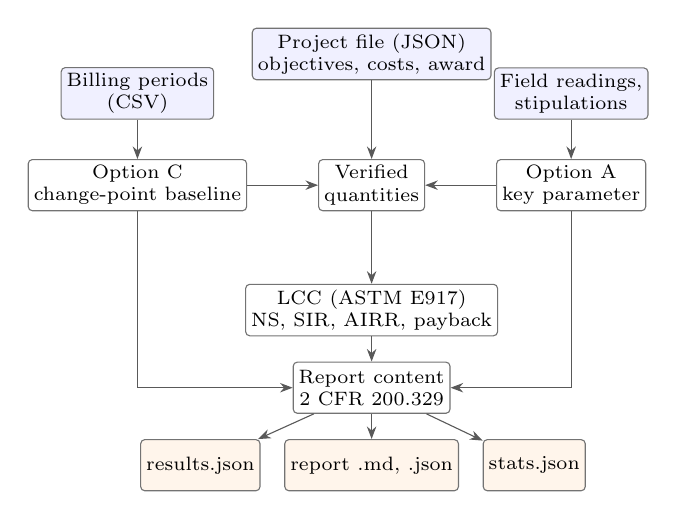
\begin{tikzpicture}[font=\scriptsize, node distance=3.2mm and 3mm,
  box/.style={draw=black!55, rounded corners=1.5pt, align=center, minimum height=6.5mm, inner sep=2pt, fill=white},
  io/.style={box, fill=blue!6},
  outb/.style={box, fill=orange!8},
  arr/.style={-{Stealth[length=1.6mm]}, black!65}]
\node[io] (proj) {Project file (JSON)\\ objectives, costs, award};
\node[box, below=10mm of proj] (q) {Verified\\ quantities};
\node[box, left=9mm of q] (c) {Option C\\ change-point baseline};
\node[box, right=9mm of q] (a) {Option A\\ key parameter};
\node[io, above=5mm of c] (csv) {Billing periods\\ (CSV)};
\node[io, above=5mm of a] (fld) {Field readings,\\ stipulations};
\node[box, below=of q, yshift=-6mm] (l) {LCC (ASTM E917)\\ NS, SIR, AIRR, payback};
\node[box, below=of l] (r) {Report content\\ 2 CFR 200.329};
\node[outb, below=of r] (o2) {report .md, .json};
\node[outb, left=3mm of o2] (o1) {results.json};
\node[outb, right=3mm of o2] (o3) {stats.json};
\draw[arr] (csv) -- (c); \draw[arr] (fld) -- (a); \draw[arr] (proj) -- (q);
\draw[arr] (c) -- (q); \draw[arr] (a) -- (q);
\draw[arr] (q) -- (l); \draw[arr] (l) -- (r);
\draw[arr] (c.south) |- (r.west); \draw[arr] (a.south) |- (r.east);
\draw[arr] (r) -- (o1); \draw[arr] (r) -- (o2); \draw[arr] (r) -- (o3);
\end{tikzpicture}
\caption{Data architecture built into MUNI-LCC. One project file and one command (\code{muni-lcc run}) produce the verified results, the life-cycle cost study computed from verified quantities, and the performance report content. The statistics file feeds the rendered documentation, and continuous integration checks that it is reproduced.}
\label{fig:arch}
\end{figure}

{\raggedright\indent
\emph{Inputs and interface.} A project is one JSON file, and any section may be omitted. Option C reads two CSV files with defined columns \code{period}, \code{days}, \code{energy}, and \code{mean\_temp}. The command \code{muni-lcc run project.json -{}-out outputs} writes \code{results.json}, \code{performance\_report.md}, and \code{performance\_report.json}; \code{muni-lcc due-date} computes a report due date alone.\par}

\emph{Traceability.} Every acceptance threshold in the configuration file contains the exact text existing from its source. The Option A module contains the measured and stipulated parameters,the basis for each stipulation, and the report repeats both simultaneously. The FEMP discount rate file records the exact source of the NIST edition.

\emph{Testing and reproducibility.} The test suite designed to validate the toolkit contains 37 tests. The test are grouped into: closed-form checks of the factors in Eqs.~(\ref{eq:spv}) to (\ref{eq:upvstar}) and of a hand-computed LCC; the NS, SIR, and AIRR identities; exact recovery of a known change-point model from noiseless data; recovery of a known injected savings fraction from noiseless and noisy data within the reported uncertainty; due dates for every reporting frequency; uncertainty reporting when savings are not positive; information-criterion selection; and an end-to-end test against the worked example's stored true answer. The worked example writes a statistics file from which the README and the software paper are rendered, and continuous integration fails if the example no longer reproduces those numbers. Every number in this study is likewise read from output files by a script (Sec.~\ref{sec:avail}).

\emph{Versions.} Version 0.1.0 was released on 14 October 2026 under the MIT license, with documentation under CC BY 4.0, and archived on Zenodo~\cite{munilcc}. This paper describes version 0.1.1, a modification of the initial version based on two changes implemented in Sec.~\ref{sec:changes} and the scripts behind this paper. Every result of the worked example in Sec.~\ref{sec:example} is identical under both versions, and continuous integration is designed to ensure this is checked for every analysis.

\section{Worked Example}\label{sec:example}

\subsection{Synthetic building and data}

The worked example built into this toolkit is a hypothetical 40,000\,ft$^2$ town hall whose natural gas boiler and controls were replaced and the initial fluorescent lighting is converted to LED. The rationale for why synthetic data are used is to ensure that the true savings are known in advance, to ensure correctness of the toolkit. With seed 2026, monthly mean temperatures are drawn as rounded illustrative values plus Gaussian jitter with a standard deviation of 2.5\,F. Based on this, the true daily gas usage is calculated as
\begin{equation}
E_{\rm true}(T)=40+6\,(58-T)^{+}\ \text{therms/day}
\label{eq:dgp}
\end{equation}
The observed usage for each month adds a Gaussian noise with a standard deviation of $\sigma=12$ therms/day. The baseline covers 24 months (2023 and 2024), and the reporting period covers 12 months (2025), where use is scaled by $1-F_{\rm true}$ with $F_{\rm true}=0.15$. The true avoided use is therefore computed as $F_{\rm true}$ times the noiseless baseline use at the reporting-period temperatures, $0.15\times\TrueAdjBaseline=\TrueAvoided$ therms. For the LED lighting measure, five circuit-demand readings before and after the retrofit have estimated means of 14.6 and 6.2 kW, and annual operating hours are stipulated at 3,380 from the posted building schedule. All prices and costs using in the worked example are invented. The applied temperatures are not NOAA normals.

\subsection{Option C baseline selection}

Table~\ref{tab:cand} compares the five candidate fits. The 3PC form is rejected because its cooling slope contains the wrong sign for a heating meter. The CV(RMSE) and BIC for the 4P and 5P forms are marginally higher than the 3PH form. Their added slopes are insignificant, so the selection rule chooses the 3PH model under either version,
\begin{equation}
\hat E(T)=\EquationIntercept+\EquationSlope\,(\EquationCp-T)^{+}\ \text{therms/day},
\end{equation}
which is relatively close to the generating model calculated in Eq.~(\ref{eq:dgp}). Therefore, this satisfy every acceptance criterion in Table~\ref{tab:accept}, and the 24-month baseline is a whole-year set. Fig.~\ref{fig:baseline} illustrates the fit.

\begin{table}[t]
\caption{Candidate Option C baseline models for the worked example (24 months). The minimum slope $|t|$ is the smallest absolute $t$-statistic among a model's slopes; BIC is Eq.~(\ref{eq:bic}); n.s., not significant. 3PC is not listed in the table because no physically valid fit exists.}
\label{tab:cand}
\centering\small
\begin{tabular}{@{}lrrrrl@{}}
\toprule
Form & CV \% & $R^2$ & min $|t|$ & BIC & Status \\
\midrule
mean & \CvMean & \RsqMean & \TMean & \BicMean & valid \\
2P & \CvTwoP & \RsqTwoP & \TTwoP & \BicTwoP & valid \\
3PH & \CvThreePH & \RsqThreePH & \TThreePH & \BicThreePH & \textbf{selected} \\
4P & \CvFourP & \RsqFourP & \TFourP & \BicFourP & slope n.s. \\
5P & \CvFiveP & \RsqFiveP & \TFiveP & \BicFiveP & slope n.s. \\
\bottomrule
\end{tabular}
\end{table}

\begin{figure}[t]
\centering
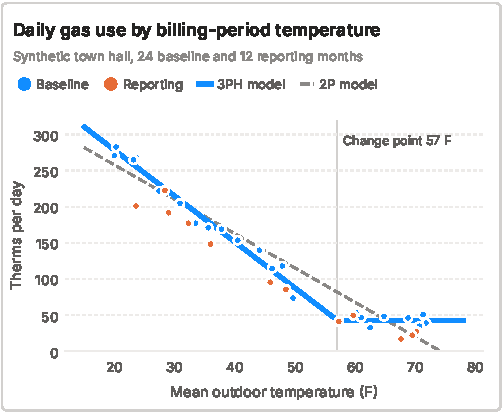
\includegraphics[width=\columnwidth]{figs/fig_baseline.pdf}
\caption{Daily gas use against mean billing-period temperature for the synthetic town hall. The blue datapoints represents the 24 baseline months while the orange datapoints are the 12 reporting months. The selected 3PH baseline (solid) captures the flat base load above the change point that the 2P fit (dashed) misses. The vertical gap between the reporting months and the baseline is the avoided energy use.}
\label{fig:baseline}
\end{figure}

\subsection{Avoided energy use and its uncertainty}

Table~\ref{tab:bench} compares the results with the already known truth. The adjusted baseline for the reporting year is \AdjBaseline{} therms and metered use is \ReportingUse{} therms, so the avoided energy use is \AvoidedTherms{} therms, or \FracSav\% of the adjusted baseline. The true value is \TrueAvoided{} therms; the error of \ErrTherms{} therms (\ErrPct\%) lies within the 90\% uncertainty of $\pm$\AbsUnc{} therms (FSU \FSU\%). Fig.~\ref{fig:monthly} shows the monthly results. The monthly differences include meter noise, justifying the wide variation between individual months although September shows slightly negative savings. The annual total is the quantity as described by the uncertainty.

\begin{table}[t]
\caption{Worked example results as compared with the known truth. Option C uses a 90\% confidence level.}
\label{tab:bench}
\centering\small
\begin{tabular}{@{}lrr@{}}
\toprule
Quantity & MUNI-LCC & Truth \\
\midrule
Option C model & \ModelForm & 3PH \\
Change point (F) & \EquationCp & 58 \\
Adjusted baseline (therms) & \AdjBaseline & \TrueAdjBaseline \\
Avoided energy use (therms) & \AvoidedTherms & \TrueAvoided \\
Fractional savings (\%) & \FracSav & 15.0 \\
90\% uncertainty (therms) & $\pm$\AbsUnc & \\
FSU at 90\% (\%) & \FSU & \\
Option A savings (kWh/yr) & \OptASavings & \OptASavings \\
Option A 90\% uncertainty (kWh/yr) & $\pm$\OptAUnc & \\
\bottomrule
\end{tabular}
\end{table}

\begin{figure}[t]
\centering
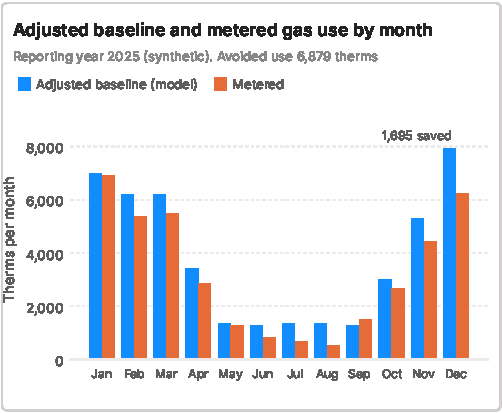
\includegraphics[width=\columnwidth]{figs/fig_monthly.pdf}
\caption{Adjusted baseline (model applied to 2025 temperatures) and metered use by reporting month. The difference summed over the year is the avoided energy use, \AvoidedTherms{} therms. The label marks the month with the largest difference.}
\label{fig:monthly}
\end{figure}

\subsection{Option A lighting savings}

From Eq.~(\ref{eq:opta}), $(14.6-6.2)\,\text{kW}\times3{,}380\,\text{h}=\OptASavings$\,kWh per year, with a measurement uncertainty of $\pm$\OptAUnc{} kWh (\OptARel\%) at 90\% confidence. The estimate equals the true value exactly, but this is based on construction rather than evidence of accuracy because the synthetic readings were chosen with estimated means of exactly 14.6 and 6.2\,kW, and the truth is defined from the same means and the same stipulated hours. However, Sec.~\ref{sec:val_a} tests the Option A uncertainty properly.

\subsection{Life-cycle cost from verified quantities}

The LCC study compares two scenarios between retaining the existing boiler and fluorescent lighting (base case) with the retrofit (alternative) over 25 years period at the FEMP 2025 real discount rate of 3.0\%. Gas and lighting quantities are drawn from the verified results as described in Sec.~\ref{sec:link}, at invented prices of \$1.20 per therm and \$0.17 per kWh. For the base case, an end-of-life boiler replacement of \$95,000 is anticipated in year 8. In the alternative case, an LED driver replacement of \$12,000 is anticipated in year 15 and a residual boiler value of \$20,000 in year 25. Table~\ref{tab:lcc} gives the breakdown. The retrofit has net savings of \$\NetSavings, an SIR of \SIR, an AIRR of \AIRR\%, a simple payback of \SPB{} years, and a discounted payback of \DPB{} years.

\begin{table}[t]
\caption{LCC breakdown for the worked example (present value, 2025 dollars; 25 years; 3.0\% real discount rate).}
\label{tab:lcc}
\centering\small
\begin{tabular}{@{}lrr@{}}
\toprule
Component & Base case & Retrofit \\
\midrule
Initial investment & \LccBInitial & \LccAInitial \\
Replacements & \LccBReplacement & \LccAReplacement \\
Residual value ($-$) & \LccBResidual & \LccAResidual \\
Energy (verified quantities) & \LccBEnergy & \LccAEnergy \\
OM\&R & \LccBOmr & \LccAOmr \\
\midrule
LCC & \LccBTotal & \LccATotal \\
\midrule
Net savings & \multicolumn{2}{r}{\NetSavings} \\
SIR; AIRR & \multicolumn{2}{r}{\SIR; \AIRR\%} \\
Payback, simple; discounted & \multicolumn{2}{r}{\SPB{} y; \DPB{} y} \\
\bottomrule
\end{tabular}
\end{table}

\subsection{Performance report content}

The award used in this worked example scenario has an annual reporting period ending 31 December 2025, which implies the report submission is due on \DueDate{} at 11:59PM. The award has three principal objectives guiding the accomplishments. Objective O1: 7,000 therms per year of avoided gas use - the results attains \OnePct\% of target and is reported as target not met, with the user's explanation attached (the controls for one heating zone were commissioned in March). Objective O2: 25,000 kWh per year of lighting savings - the result attains \TwoPct\% of target, an indicator that target is met and exceeded. Objective O3: positive net savings, is met. Project actual cost exceeds the \$185,000 budget by \$11,500, so the report contains an explanation for the cost overrun. The actual unit cost on a verified basis is \$\ActualUnit{} per first-year therm avoided against a planned \$\PlannedUnit, \UnitRatio\% higher, which is within the 10\% tolerance and is not flagged as a high unit cost. The completeness check finds no missing explanations.

\section{Validation and Sensitivity}\label{sec:validation}

A single worked example applied in this study illustrates that the computation recovers a known answer once. However, the results do not establish the accuracy of the uncertainty stated. To ensure accuracy of results, this section performs multiple replications of the example's data-generating process, varies its input, and investigates how often the reported 90\% band contains the true value of the avoided energy use. It also varies the life-cycle cost inputs. All analysis use the latest version 0.1.1 with its default model forms, selection rule, and acceptance criteria; Sec.~\ref{sec:changes} compares the results with version 0.1.0 on identical data. The scripts are described in Sec.~\ref{sec:avail}.

\subsection{Monte Carlo coverage of the Option C uncertainty}\label{sec:val_c}

\emph{Design.} Each replication draws a new 24-month baseline and 12-month reporting period from Eq.~(\ref{eq:dgp}) with the reference settings of Sec.~\ref{sec:example} ($F_{\rm true}=0.15$, $\sigma=12$ therms/day, temperature jitter 2.5\,F). It runs the entire Option C procedure and records the estimate $S_C$, the reported half-width $U_C$ at 80\%, 90\%, and 95\% confidence, the selected form, and the acceptance outcome. The truth in each replication is calculated as $F_{\rm true}$ times the noiseless baseline use at that replication's reporting temperatures. A replication is covered when $|S_C-S_{\rm true}|\le U_C$. For \McReps{} replications, the Monte Carlo standard error of a coverage near 90\% is about \McSeRef{} percentage points.

\emph{Results.} The estimator shows no detectable bias: the mean error is \McMeanErr{} therms against a mean true saving of \McMeanTrue{} therms, and the root-mean-square error is \McRmse{} therms. Empirical coverage is \McCovEighty\%, \McCovNinety\%, and \McCovNinetyFive\% at nominal 80\%, 90\%, and 95\%, each within about one Monte Carlo standard error of nominal (Fig.~\ref{fig:mc}). For monthly data generated without autocorrelation, the ASHRAE Guideline 14 approximation in Eq.~(\ref{eq:fsu}) is therefore well calibrated in this setting. This is consistent with the position that the approximation's known shortfalls arise mainly from autocorrelated residuals in daily and hourly models~\cite{touzani2019}, which this test does not include.

\begin{figure*}[t]
\centering
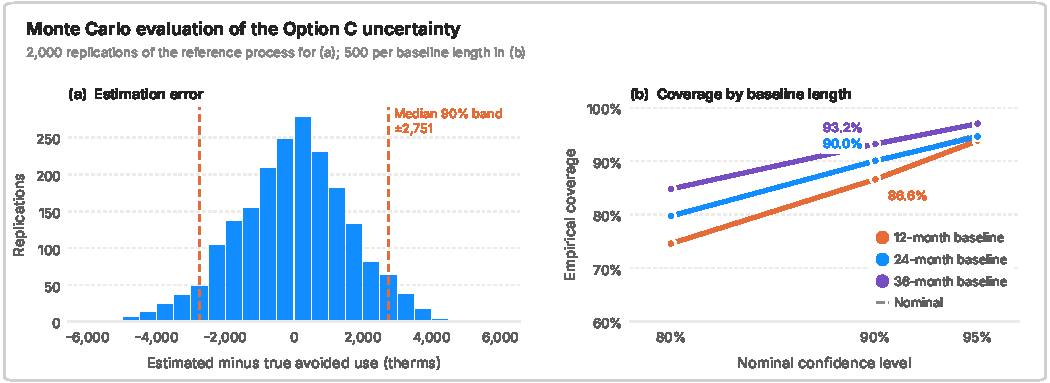
\includegraphics[width=\textwidth]{figs/fig_mc.pdf}
\caption{Monte Carlo evaluation of Option C. (a) Distribution of estimation error over \McReps{} replications of the reference process (bins of 500 therms); dashed lines mark the median reported 90\% half-width. (b) Empirical coverage of the reported uncertainty against the nominal confidence level for 12-, 24-, and 36-month baselines. The 24-month reference uses \McReps{} replications and the other two use \ScanReps{} each.}
\label{fig:mc}
\end{figure*}

\emph{Model selection.} The generating model is 3PH, and the selection rule chooses 3PH in \McFormThreePH\% of replications, 4P in \McFormFourP\%, and 5P in \McFormFiveP\%. The remaining over-parameterized choices occur when an extra slope passes the $|t|>2$ screen and also lowers the BIC, which happens by chance in a minority of noisy baselines. Coverage is \CovFormThreePH\% in the replications where 3PH is selected and \CovFormFourP\% where 4P is selected.

\emph{Acceptance outcomes.} Every replication passes the $R^2$, NMBE, slope-$t$, and CV(RMSE) criteria (median CV(RMSE) \McMedCv\%), and NMBE never exceeds $\McMaxNmbe$ percent, confirming that it is zero by construction under days-weighted least squares (Sec.~\ref{sec:optc}). This validation confirms that the NMBE criterion cannot fail for fits produced by the toolkit. The binding criterion is FSU: \McPass\% of replications pass all criteria, and every failure is an FSU above 50\%. The worked example's FSU of \FSU\% is therefore not unusual; the median over replications is \McMedFsu\%.

\subsection{Changes in version 0.1.1}\label{sec:changes}

The same tests were initially conducted on version 0.1.0 where two behaviors were identified and corrected in Version 0.1.1. Table~\ref{tab:changes} compares both versions from identical data.

\emph{Model selection.} Version 0.1.0 selected the significant-slope model using the lowest CV(RMSE). For the reference process, it chose a 4P or 5P model in \BeforeNonThree\% of replications. Since each slope's $t$-statistic is computed conditional on a change point that was chosen to minimize error, the $|t|>2$ screen admits a spurious slope more often than its nominal level implies, and CV(RMSE) penalizes an added parameter only through $n-p$. The over-fitted models reported a lower CV(RMSE) and understated their own uncertainty. With selections by BIC, Eq.~(\ref{eq:bic}), penalizes each added parameter by $\ln n$. It reduced the over-parameterized choices to \AfterNonThree\%, raised coverage at 90\% from \BeforeCovNinety\% to \McCovNinety\%, and lowered the RMSE from \BeforeRmse{} to \McRmse{} therms. To ascertain that the stricter rule does not underfit, the test was repeated on processes whose true model is 4P or 5P. For a true 4P model the two rules perform alike. For a true 5P model, BIC identifies the 5P form less often (\UfFivePAfter\% against \UfFivePBefore\%), but the RMSE of the savings estimate changed by only \UfFivePRmseChange\% and coverage is \UfFivePCovAfter\% against \UfFivePCovBefore\%. For this process, the effect on the savings estimate is considerably small.

\emph{Uncertainty for non-positive savings.} Version 0.1.0 computed the absolute uncertainty as FSU times savings and therefore reported none when estimated savings were zero or negative, which occurred in \BeforeUndefFive\% of replications at 5\% true savings. Version 0.1.1 computes $U_C$ directly from Eq.~(\ref{eq:uc}), which does not involve savings, so a report can state that savings were not distinguishable from zero. Coverage at 5\% true savings rises from \BeforeCovFive\% to \CovFrFive\%, and at $\sigma=36$ from \BeforeCovNoise\% to \CovNoiseThirtySix\%.

Neither change affects the worked example: its candidate models rank the same under both rules highlighted in (Table~\ref{tab:cand}), and its savings are positive.

\begin{table}[t]
\caption{Option C results based on identical synthetic data under versions 0.1.0 and 0.1.1. The reference process has a true 3PH model ($F_{\rm true}=15\%$, $\sigma=12$ therms/day, 24-month baseline, \McReps{} replications); the weak and noisy rows use \ScanReps{} replications each.}
\label{tab:changes}
\centering\small
\begin{tabular}{@{}lrr@{}}
\toprule
 & v0.1.0 & v0.1.1 \\
\midrule
\multicolumn{3}{@{}l}{\emph{Reference process, true model 3PH}} \\
\BeforeAfterRows
\bottomrule
\end{tabular}
\end{table}

\subsection{Dependence on savings size, noise, and baseline length}

Table~\ref{tab:scan} varies one setting at a time with \ScanReps{} replications each (Monte Carlo standard error about \McSeScan{} points at 90\%). Within each block the same random draws are reused across settings, so differences between rows reflect the setting rather than sampling.

\begin{table*}[t]
\caption{Option C performance as one setting is varied from the reference ($F_{\rm true}=15\%$, $\sigma=12$ therms/day, 24-month baseline). Errors are in therms. Coverage is the share of replications in which the reported band contains the truth. The last column is the share of replications where the estimated savings are zero or negative; the absolute uncertainty is still reported for them, but FSU is not, and they fail the FSU criterion.}
\label{tab:scan}
\centering\small
\begin{tabular}{@{}lrrrrrrrr@{}}
\toprule
Setting & Mean error & RMSE & Median FSU$_{90}$ (\%) & Cov.\ 80\% & Cov.\ 90\% & Cov.\ 95\% & Pass all (\%) & $S_C\le0$ (\%) \\
\midrule
\ScanRows
\bottomrule
\end{tabular}
\end{table*}

\emph{Savings fraction.} Error and absolute uncertainty do not change with $F_{\rm true}$, as Eq.~(\ref{eq:fsu}) implies (Sec.~\ref{sec:fsu}): the RMSE is the same in every row of the block. The noticeable change in every block is the FSU, from a median of \MedFsuFive\% at 5\% savings to \MedFsuThirty\% at 30\%, together with the acceptance rate, from \PassFrTen\% at 10\% savings to \PassFrTwenty\% at 20\%. In practical applications, the FSU criterion in Table~\ref{tab:accept} determines whether a project of this size and noise level can be verified at all from monthly bills. At 5\% savings, the estimate is zero or negative in \NonposFive\% of replications; the band is still reported, and coverage is \CovFrFive\%.

\emph{Noise.} By halving the noise to $\sigma=6$, the RMSE is instantaneously halved (\RmseNoiseSix{} therms) and every replication passes. At $\sigma=36$ the RMSE is \RmseNoiseThirtySix{} therms and only \CvOkNoiseThirtySix\% of replications meet the CV(RMSE) criterion, but the coverage stays at or above nominal in all noise settings: noticeably, the band widens with the noise as it should.

\emph{Baseline length.} A 12-month baseline raises the RMSE to \RmseYrOne{} therms and lowers coverage to \CovYrOne\% at nominal 90\% and \CovYrOneEighty\% at nominal 80\%, an indicator that the approximation is somewhat optimistic for the shortest baseline acceptable by FEMP v5.0. A 36-month baseline lowers the RMSE to \RmseYrThree{} therms, and coverage of \CovYrThree\% is slightly conservative. These results support the FEMP v5.0 guidance to use whole-year baselines, suggestive that one year baseline should be treated as a minimum rather than a target.

\subsection{Option A coverage}\label{sec:val_a}

The worked example's exact Option A match is built into the example (Sec.~\ref{sec:example}). To test Eq.~(\ref{eq:opta_unc}), we drew \OaReps{} replications of five readings before and after the retrofit from normal distributions with means of 14.6 and 6.2 kW and a standard deviation of \OaSd\,kW, with the operating hours fixed at their stipulated value. Coverage is \OaCovEighty\%, \OaCovNinety\%, and \OaCovNinetyFive\% at nominal 80\%, 90\%, and 95\%, and the median relative uncertainty at 90\% is \OaMedRel\%. This result confirms the arithmetic of the interval for independent, normally distributed readings. It records no information about the uncertainty in stipulated hours, which the toolkit does not quantify by design.

\subsection{Sensitivity of the life-cycle cost results}\label{sec:val_lcc}

\emph{Propagation of measured-savings uncertainty.} Each verified therm of gas savings calculated in this replication is worth \$\NsPerTherm{} of net present value over the study period. When both verified quantities are moved to the edges of their 90\% bands (gas $\pm$\AbsUnc{} therms, lighting $\pm$\OptAUnc{} kWh), the net savings increases from \$\NsLow{} to \$\NsHigh{} and the SIR from \SirLow{} to \SirHigh. Across the band, the cost-effectiveness verdict remains unchanged across the band, but its size is uncertain by roughly a third in either direction, which a report derived from a single projected savings would not have shown.

\emph{Discount rate, energy price, and study period.} Fig.~\ref{fig:lcc} varies one input at a time for each replication. Net savings fall with the real discount rate and reach zero at \BeRate\%, where the adjusted internal rate of return (AIRR) equals the discount rate as indicated in Eq.~(\ref{eq:airr}). Net savings becomes positive in a study period of \BeYears{} years, then increases linearly with the gas price, and remains consistently positive (\$\NsZeroGas) even at a gas price of zero.

In this synthetic worked example, the avoided base-case boiler replacement and the lighting and maintenance savings exceed the added investment on their own. This further establishes that the verified gas savings worth about \$\GasSavPV{} in the present value, determine the size of the net savings rather than its positive or negative sign.

\begin{figure*}[t]
\centering
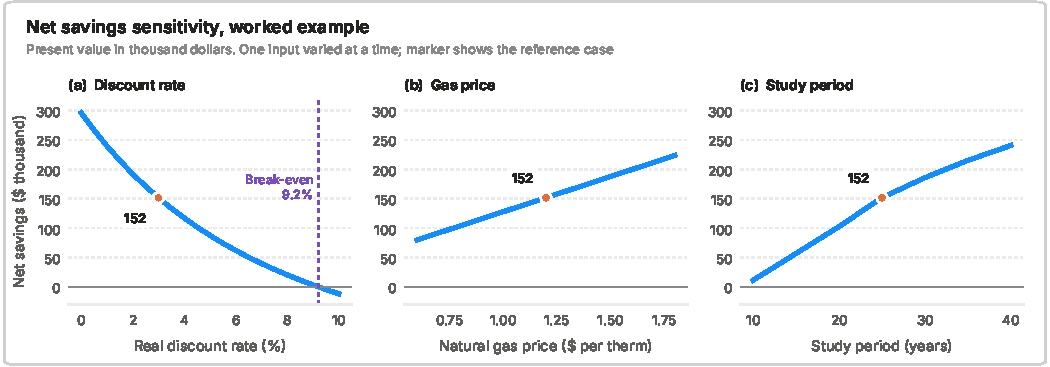
\includegraphics[width=\textwidth]{figs/fig_lcc.pdf}
\caption{Net savings of the worked example as one life-cycle cost input is varied: (a) real discount rate, (b) natural gas price, (c) study period. The orange marker is the reference case (3.0\%, \$1.20 per therm, 25 years; net savings \$\NetSavings); the dotted line in (a) marks the break-even rate.}
\label{fig:lcc}
\end{figure*}

\section{Limitations and Scope}\label{sec:limits}

There are four core measurement and verification options defined by IPMVP. Of these options, the toolkit implements two of the four IPMVP options: Options A (key parameter measurement) and C (whole facility). Option B (all parameters measured) and Option D (calibrated simulation) are not implemented in this toolkit. Option C uses temperature as the only independent variable, other variables such as occupancy, school calendars, and production are not modeled. Non-routine adjustments must be estimated outside the toolkit and documented in the M\&V plan. Avoided energy use is computed, but normalized savings is not accounted for. The uncertainty method applied is the ASHRAE Guideline 14 approximation for monthly data rather than the EVO 10100-1:2018 procedure cited in FEMP v5.0; it does not correct for autocorrelation and should not be applied to daily or hourly data without that correction~\cite{touzani2019,walter2014}. The 1.26 constant used in the toolkit has not been verified against a licensed copy of the 2023 guideline. The Monte Carlo results in Sec.~\ref{sec:validation} is based on a data-generating process that matches the 3PH model family, has independent Gaussian errors, and has no non-routine events, so they present calibration under favorable conditions. They do not represent as evidence of performance on real municipal billing data, which has not yet been tested in this toolkit. Life-cycle cost is calculated in constant dollars; taxes, financing, and incentives as cash flows are not modeled. Finally, the report module organizes the content as specified in 2 CFR 200.329 and checks its completeness. It is not a compliance determination procedure and does not replace the form prescribed by the awarding agency, and it does not model due-date extensions.

\section{Concluding Remarks}\label{sec:conclusion}

MUNI-LCC is a compact open access toolkit designed to implement the performance reporting process for energy efficiency upgrades, from metered data to a federal performance report based on IPMVP Options A and C as defined in FEMP v5.0, life-cycle cost consistent with ASTM E917, and content elements of 2 CFR 200.329. The integral essence for the development of the toolkit is to ensure that verified quantities, not projections, are computed into the life-cycle cost study so that Net Savings (NS), Savings-to-Investment Ratio (SIR), Adjusted Internal Rate of Return (AIRR), and unit cost are accurately reported on a measured basis with every acceptance value referencing its source.

Based on observation from the synthetic example with a known answer, it is confirmed that the toolkit recovers the injected gas savings within its stated uncertainty. Across \McReps{} replications of the same process, the Option C uncertainty attains coverage of \McCovNinety\% at a nominal 90\% with no detectable bias, and Option A coverage is likewise close to nominal. Findings from the tests in version 0.1.0 justified the need for two changes which was implemented in version 0.1.1. The two changes include: model selection by information criterion, which cuts spurious change-point models from \BeforeNonThree\% to \AfterNonThree\% of replications; and an absolute uncertainty reported for any sign of savings. Neither of these changes altered the worked example. The tests further validate that the FSU criterion, not the model fit, decides whether a modest saving can be verified from the monthly bills.

Future scope of work will include the integration of Option B (all parameter measurement), the EVO 10100-1:2018 uncertainty procedure alongside the current approximation, normalized savings, and additional independent variables, validated against real municipal billing data compared against an established open M\&V implementation on the same data.

\section*{Code and Data Availability}\label{sec:avail}

The MUNI-LCC source code, documentation, synthetic example data, and tests are packaged in a repository publicly accessible at \url{https://github.com/Olumide-Akindipe/muni-lcc} under the MIT license (documentation CC BY 4.0). The manuscript source and the scripts supporting every table and figure in this paper (\code{validation.py}, \code{underfit\_check.py}, \code{lcc\_scans.py}, \code{figures.py}, and \code{make\_numbers.py}, which writes every number in the text from the output files) are in the \code{preprint/} folder of the repository, together with their outputs. Version 0.1.0 is archived on Zenodo~\cite{munilcc}, and every version, including 0.1.1, is available under the concept DOI 10.5281/zenodo.23362541. Real utility data are not used.

\section*{Competing Interests}

The author declares no competing interests.

\section*{Acknowledgment}

No financial support was received for this work.

\bibliographystyle{unsrtnat}
\bibliography{refs}


\end{document}
